% !TEX root = ../macro.tex
\section{Understanding Economic Fluctuations}\label{sec:fluctuations-intuition}

A factory receives fewer orders. At first it reduces overtime and lets
inventories rise. If weak sales continue, it postpones equipment purchases
and stops recruiting. Its suppliers lose business; some workers reduce
spending. The factory's machines and its workers' skills have not suddenly
vanished, yet production, income, and employment can change together.

This is a useful starting puzzle. What changed first? Why did other people
respond? Why did adjustment take time? And when orders recover, will the
economy simply return to its former path? The factory is a teaching example,
not an explanation of every recession. It lets us construct the questions
before choosing between competing models of the answers.

\subsection{Why study growth before fluctuations?}

The order in these notes is an analytical convenience, not a rule that
all courses follow or that economies obey. Growth theory first gives us
an account of productive resources, accumulation, consumption choices,
and intertemporal consistency. We can then ask how those choices respond
when conditions change unexpectedly or adjustment is incomplete.

A household facing a temporary income loss still compares consumption
today with future opportunities. A firm revising investment still inherits
its existing capital. A government trying to stabilize activity still
uses resources or reallocates claims on resources. The growth models
establish these relationships before uncertainty, labor adjustment, nominal
contracts, and financial constraints complicate their interaction.

This sequence also provides benchmarks. To say that output is unusually
weak, we need to specify weak relative to what: its previous level, an
estimated trend, a forecast made before the disturbance, or a model's
feasible or efficient allocation. Growth theory helps us think about the
benchmark; it does not make that benchmark observable or immune to shocks.

Historically and conceptually, growth and fluctuations also pose joint
questions. A period of weak activity can change investment, skills, entry,
and innovation. A change in expected future productivity can change spending
today. Studying a deterministic growth model first isolates some mechanisms;
it does not imply that growth happens first in calendar time or independently
of the disturbances that arrive along the way.

\Needspace{11\baselineskip}
\begin{greenblock}
\textbf{Growth gives us a path and a structure; fluctuations ask how they move.}
Carry forward the inherited stocks, budgets, and choices. Then ask what
changed, what can adjust now, and what must adjust later. A useful benchmark
need not be a fixed trend, and a fluctuation need not leave that benchmark
unchanged.
\end{greenblock}

\subsection{What exactly are we describing as a fluctuation?}

We use economic fluctuations to describe uneven movements in aggregate
production, spending, employment, and related variables over time. The
object is a joint economic episode, not necessarily a deviation from one
fixed smooth line. Begin with the observed movements before assigning them
to a trend, a cycle, or a particular cause.

\subsubsection{Levels, growth rates, and deviations answer different questions}

Let $Y_t>0$ denote real output measured consistently across dates. The
log growth rate is $\Delta\log Y_t=\log Y_t-\log Y_{t-1}$. If output
rises from 100 to 105 and then to 107, growth slows but output does not fall.
If output instead falls from 100 to 95 and then rises to 98, the final
period has positive growth but output remains below its initial level.
Returning from 95 to 100 requires an increase of about 5.26\%, not 5\%.
These are arithmetic examples, not recession-dating rules.

For a chosen reference path $\bar Y_t>0$, define a log deviation
\[
d_t=\log Y_t-\log\bar Y_t.
\]
It is approximately the proportional deviation for small gaps. It can be
negative while actual output is growing: a growing economy can lag behind
an even faster-growing reference path. Conversely, output can fall and
still lie above a chosen reference. The sign of growth and the sign of
the deviation are different descriptions.

There are several possible references, with different interpretations.
\Needspace{20\baselineskip}
\begin{center}
\small
\begin{tabular}{p{0.25\linewidth}p{0.30\linewidth}p{0.31\linewidth}}
\hline
\tableheading{Reference} & \tableheading{What the comparison asks} & \tableheading{What it does not establish}\\
\hline
Previous peak & Has the previous level of activity been regained? &
Whether the economy has caught up with a growing counterfactual path\\[4pt]
Statistical trend & How far is output from a fitted smooth component? &
That the smooth component is productive capacity or an efficient allocation\\[4pt]
Earlier forecast & How far is activity from the path previously expected? &
That every forecast error is an inefficient output loss\\[4pt]
Model benchmark & How does output compare with the stated model allocation? &
That the model's technology, frictions, or welfare criterion fit the episode\\
\hline
\end{tabular}
\end{center}

Potential output is an estimate of sustainable production under specified
conditions. Natural output often denotes a model's flexible-price allocation
under the other stated frictions; efficient output uses a welfare criterion.
These need not coincide. A statistical filter cannot establish their equality.
The reference must be named before a deviation is interpreted as slack,
overheating, or a welfare loss.

Detrending is therefore part of the measurement problem. The estimated
trend can change when new data arrive, especially near the end of the
sample; an actual change in trend can also be assigned to the cycle by
an unsuitable method. Hamilton's critique of the HP filter illustrates
how detrending can introduce misleading dynamics.\footnote{James D.
Hamilton (2018), ``Why You Should Never Use the Hodrick--Prescott Filter,''
\textit{Review of Economics and Statistics}, 100(5), 831--843; working-paper
version: \url{https://www.nber.org/papers/w23429}. The methodological lesson
here is to examine the decomposition, not to presume that another filter
reveals the true economic benchmark.}
For a first description, report the actual path alongside the deviation
and explain how the reference was constructed.

\subsubsection{An aggregate episode has breadth, timing, and composition}

A decline at one firm is not automatically an aggregate recession. It
might reflect customers moving to a competitor, a seasonal lull, or a
sector shrinking while another expands. The business-cycle question is
why activity moves across many firms, sectors, or households, and how
those movements relate to one another.

Describe the amplitude of a movement, its duration, and its persistence.
Then examine comovement: do employment, hours, consumption, investment,
and output move together or in opposite directions? Timing matters too.
Orders, production, hiring, unemployment, and wages need not turn at the
same date. A variable is called procyclical or countercyclical relative
to a stated activity measure; leading and lagging describe timing, not
causation.

Stock and Watson's study of postwar US macroeconomic time series organizes
the evidence around these kinds of relationships.\footnote{James H. Stock
and Mark W. Watson (1999), ``Business Cycle Fluctuations in US Macroeconomic
Time Series,'' \textit{Handbook of Macroeconomics}, 1A, 3--64;
working-paper version: \url{https://www.nber.org/papers/w6528}. The data
coverage is historical US evidence, not a claim of identical regularities
in every country or period.}
Consumption categories should also be separated: a household may postpone
a car purchase while maintaining food consumption. Investment and durable
purchases can move sharply because their timing is adjustable. A story
about aggregate consumption that ignores this composition may miss the
margin on which households respond.

Before interpreting a series, specify whether it is real or nominal,
aggregate or per person, and seasonally adjusted where appropriate.
Predictable holiday spending is different from an unexpected demand change.
A rise in nominal sales can reflect higher prices rather than more goods.
A revision to GDP estimates can change our description without changing
what firms actually produced at the time.

\subsubsection{A business cycle is not a regular clock}

Expansion, peak, contraction, and trough describe phases of aggregate
activity. They do not require a repeating sine wave or a known period.
An economy can be hit again before it has adjusted to an earlier disturbance.
Different sectors and countries can also move at different times.

For US recession dating, the NBER considers the size, breadth, and duration
of declines across several indicators. Its chronology is not mechanically
the rule of two consecutive quarters of falling real GDP.\footnote{NBER,
``Business Cycle Dating Procedure: Frequently Asked Questions,'' explains
its US chronology, indicators, and treatment of depth, diffusion, and duration.
\href{https://www.nber.org/research/business-cycle-dating/business-cycle-dating-procedure-frequently-asked-questions}{NBER dating FAQ}.}
A trough marks a turning point into expansion; it does not certify that
employment, household incomes, or output relative to a previous forecast
have recovered. Other countries and institutions may use different dating
procedures. Keep the descriptive convention separate from the explanation.

\subsection{Where can fluctuations come from?}

\subsubsection{Begin with the first change in opportunities, spending, or financing}

Return to the factory. Fewer orders could begin with a buyer losing income,
a rise in financing costs, or a decision to postpone purchases. Output could
also fall because an essential input becomes unavailable, even when buyers
still want the product. Similar observed production declines can begin from
different changes in the economic environment.

\Needspace{28\baselineskip}
\begin{center}
\small
\begin{tabular}{p{0.22\linewidth}p{0.31\linewidth}p{0.33\linewidth}}
\hline
\tableheading{Starting disturbance} & \tableheading{Concrete situation} & \tableheading{First question for the mechanism}\\
\hline
Production or input availability & A component shortage prevents assembly;
energy becomes more costly & Which feasible production opportunities or marginal costs changed?\\[4pt]
Private spending & Households postpone durable purchases; firms revise expected sales &
Why did desired spending change at the existing prices and incomes?\\[4pt]
Financing and balance sheets & Lenders cut credit limits; collateral loses value &
Who cannot fund a planned transaction, and which losses or constraints caused it?\\[4pt]
Policy & The policy rate, taxes, purchases, or a regulatory rule changes &
Which part was anticipated or a response to economic conditions?\\[4pt]
News and uncertainty & A future technology improvement is announced;
income risk becomes harder to assess & Which expectations or risks changed before current production did?\\[4pt]
Reallocation & Demand shifts between sectors needing different skills or equipment &
How costly is moving people and resources to the new uses?\\
\hline
\end{tabular}
\end{center}

These categories overlap. An input shortage can reduce household income
and spending. Lower asset prices can reflect worse expected profits, then
reduce collateral and restrict credit. A rise in uncertainty can encourage
some households to build buffers or some firms to delay irreversible
projects, with the direction and size depending on preferences, constraints,
and available options. A label identifies a candidate channel, not a complete
causal account.

\subsubsection{A shock is defined relative to information and a model}

In a model, a shock commonly means a new realization or innovation that
was not predicted from the information available at the previous decision
date. The level of a tax, productivity, or an interest rate is not itself
necessarily a shock. A policy action can partly be a predictable response
to inflation or activity; interpreting the whole action as an independent
policy disturbance would confuse response with cause.

An anticipated future change can affect activity before its implementation.
If a buyer expects new equipment to be much better next year, today's orders
may change now. The new information arrives today, even though the physical
improvement occurs later. Rational expectations, where assumed, do not mean
that agents foresee every realization or agree that nothing can go wrong.

Exogeneity is also a modeling boundary. A foreign demand change can be
external to a small region while being the outcome of households and firms
in the rest of the world. A productivity residual may reflect utilization
or measurement, as well as technology. Calling a residual a technology shock
does not identify its economic source.

Some models generate fluctuations through feedback, delayed adjustment,
financial fragility, or changes in expectations without a sequence of large
external disturbances. Self-fulfilling expectations require conditions such
as strategic complementarities and an equilibrium-selection account; they
cannot be inferred merely because confidence and activity fall together.
A stable deterministic model without such mechanisms will not start cycling
simply because its agents make choices.

\Needspace{11\baselineskip}
\begin{blueblock}
\textbf{An observed surprise is not yet an identified cause.}
A forecast error says that the outcome differed from an expectation.
A structural explanation specifies the change in opportunities, preferences,
constraints, information, or policy that produced it. Identification asks
what evidence separates that explanation from competing changes occurring
at the same time.
\end{blueblock}

\subsection{How does a disturbance become an aggregate movement?}

\subsubsection{Separate the impulse from propagation and amplification}

The impulse is the initiating change. Propagation is how its effects move
across time, sectors, and people. Amplification means that interactions make
the response larger than a specified direct-effect comparison. Persistence
means that the response remains after the initiating innovation; it need
not imply periodic oscillation.

A missing component interrupts a producer. Its customers then face delays,
its suppliers lose orders, and its workers may lose income. Networks make
a local disturbance relevant elsewhere. A customer who postpones a purchase
reduces a seller's revenue; if that seller cuts wages or jobs and the affected
households cannot smooth consumption, another round of spending can fall.
The strength of this feedback depends on price adjustment, alternative
buyers, insurance, financial access, and policy responses.

Falling collateral can create another loop. A borrower loses funding,
reduces purchases or sells assets, and those sales can further reduce asset
prices under limited market absorption. Conversely, buffers, insurance,
flexible substitution, and stabilizing policy can damp a disturbance.
The initiating shock and the strength of these loops are separate objects.

A small disturbance can therefore produce a large movement in one setting
and a modest movement in another. But a large observed decline does not
prove a multiplier or a financial accelerator: the initiating disturbance
might itself have been large. The direct effect, the comparison economy,
and the feedback must be specified.

\subsubsection{A temporary innovation can have a persistent response}

A deliberately simple recursion makes the timing distinction visible:
\[
x_t=\rho x_{t-1}+\varepsilon_t,\qquad 0\leq\rho<1.
\]
Here $x_t$ is a dimensionless activity deviation, $\rho$ is an assumed
persistence coefficient, and $\varepsilon_t$ is an innovation. Start from
$x_{-1}=0$, set $\varepsilon_0=-1$, and set every later innovation to zero.
Substitution gives
\[
x_0=-1,\qquad x_1=-\rho,\qquad x_2=-\rho^2,
\qquad x_t=-\rho^t\quad(t\geq1).
\]
The innovation lasts one period. Unless $\rho=0$, its response lasts longer.
Higher $\rho$ slows its decay; these paths do not repeatedly change sign.
This is a timing illustration, not a household problem, an estimated response,
or proof of a particular source of persistence. In a structural model,
capital, job matching, contracts, or balance sheets would have to generate
the relevant dynamics.

\begin{figure}[!ht]
\centering
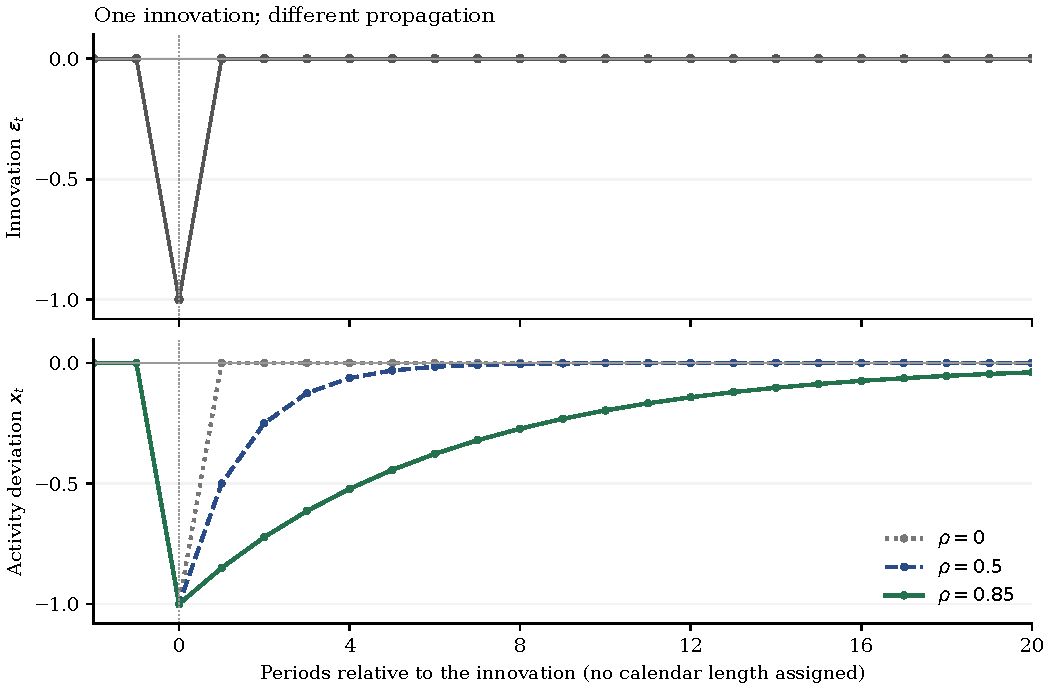
\includegraphics[width=\linewidth]{fluctuation_impulse_propagation.pdf}
\caption{The same one-period negative innovation with different assumed
persistence coefficients. All paths have the same impact. The lower panel
shows subsequent activity, not additional shocks. Periods have no assigned
calendar length, and the curves are not estimates.}
\label{fig:fluctuation-propagation}
\end{figure}

The accumulated deviation in this stable example is
$\sum_{t=0}^{\infty}x_t=-1/(1-\rho)$. That is an area in units of the
chosen deviation, not a welfare measure or an identified amount of GDP lost.
It shows why impact size alone is insufficient to describe a disturbance.
Figure~\ref{fig:fluctuation-propagation} holds the impact fixed to isolate
persistence; a full model can change impact and duration together.

\subsubsection{Individual plans meet through income, prices, and constraints}

A household can try to improve its finances by spending less. If many
households do so together, their suppliers' revenues change. It is then
necessary to explain how saving reaches investment, how prices and interest
rates respond, and whether output or employment adjusts. Planned saving
is not an extra stock of goods available independently of those responses.

In a flexible-price economy with effective intermediation, some adjustment
may occur through relative prices and intertemporal substitution. With
sticky prices, pessimistic expected sales, or binding financing constraints,
the same initial spending intention can produce a different output response.
The paradox of thrift is a conditional general-equilibrium mechanism, not
a statement that saving is always harmful. It is consistent with the growth
chapters' finding that accumulation can improve future opportunities.

The same principle applies to a firm cutting wages or costs: an individually
sensible response changes other people's income and choices. Individual
optimization does not by itself guarantee an efficient aggregate outcome
when externalities or other distortions are present. Conversely, adjustment
to a genuinely reduced production opportunity can lower output even in an
efficient equilibrium. Falling output alone does not choose between these
accounts.

\subsection{Do fluctuations belong to the short, medium, or long run?}

\subsubsection{The relevant clock is the adjustment mechanism}

Business-cycle analysis often focuses on changes over quarters and years.
That is a useful scale for production, spending, and employment decisions;
it is not a definition that all effects expire within a fixed number of years.
Short, medium, and long run describe which adjustments have had time to
occur. Those adjustments overlap rather than occupying sealed calendar boxes.

\Needspace{23\baselineskip}
\begin{center}
\small
\begin{tabular}{p{0.18\linewidth}p{0.34\linewidth}p{0.34\linewidth}}
\hline
\tableheading{Perspective} & \tableheading{Adjustments to examine} & \tableheading{Why an effect may remain}\\
\hline
Short run & Orders, inventories, hours, spending, prices, and contracts &
Existing commitments or constraints can prevent immediate reallocation\\[4pt]
Medium run & Hiring, matching, capital installation, sectoral movement, and debt repair &
Stocks, skills, and financial positions take time to rebuild or reorganize\\[4pt]
Long run & Productive capacity, institutions, research, and paths of technology and population &
Earlier decisions can alter the stocks or accumulation mechanisms that support later activity\\
\hline
\end{tabular}
\end{center}

A price can change quickly while a borrower remains heavily indebted.
Construction can stop immediately although an unfinished plant takes years
to repurpose. Employment can recover in aggregate while displaced workers
still need different skills. The appropriate horizon depends on the question
and the constraints that remain, not simply on how much time has passed.

Financial movements can also have a different timescale from measured
business-cycle movements. Drehmann, Borio, and Tsatsaronis (2012) document
longer movements in credit and property prices in their historical financial-
cycle analysis.\footnote{Mathias Drehmann, Claudio Borio, and Kostas
Tsatsaronis (2012), ``Characterising the Financial Cycle: Don't Lose Sight
of the Medium Term!'' \textit{BIS Working Papers}, no.~380.
\url{https://www.bis.org/publ/work380.htm}. This is evidence under that
paper's definition and sample, not a universal period for every credit cycle.}
A short recovery in spending need not complete balance-sheet repair. Nor
does a longer financial movement establish that every business cycle began
in finance.

\subsubsection{Shock duration, recovery time, and lasting damage are different}

A shipping interruption might end quickly while inventories, production
schedules, and customers' orders take longer to normalize. A persistent
rise in energy costs may require a new production mix instead of restoration
of the old one. A brief period without credit might close a firm whose
customer relationships cannot be recreated immediately.

The growth chapters make these links explicit. Less investment changes
future capital. Less training can change skills. Research cuts or reduced
entry can change later innovation. Not every temporary reduction produces
a permanent effect: replacement investment, rehiring, catch-up, or new entry
can restore the previous path under suitable conditions. The adjustment
mechanism must determine whether and how that happens.

In the strict sense, hysteresis means that history changes the economy's
long-run outcome, rather than merely producing slow convergence to the same
one. Blanchard and Summers' analysis of European unemployment is a classic
application of this idea.\footnote{Olivier J. Blanchard and Lawrence H.
Summers (1986), ``Hysteresis and the European Unemployment Problem,''
\textit{NBER Macroeconomics Annual}, 1, 15--78; working-paper version:
\url{https://www.nber.org/papers/w1950}.}
The term should not substitute for a mechanism. Lost skills, disrupted job
matching, and a temporary hiring delay have different implications for
whether an effect eventually disappears.

Cerra and Saxena (2008) provide historical cross-country evidence of highly
persistent output losses after financial crises and some political crises.
\footnote{Valerie Cerra and Sweta Chaman Saxena (2008), ``Growth Dynamics:
The Myth of Economic Recovery,'' \textit{American Economic Review}, 98(1),
439--457. \url{https://doi.org/10.1257/aer.98.1.439}. The statement concerns
the crises and methods studied there, not an inevitability for every downturn.}
This is a reason to investigate lasting losses, not permission to label every
estimated trend break as the causal effect of a recession. The earlier
forecast may have been too optimistic, and the disturbance may itself have
changed productive opportunities.

\Needspace{11\baselineskip}
\begin{blueblock}
\textbf{Long-run adjustment does not mean returning to the old forecast.}
A model can have flexible prices in the long run and still inherit different
capital, skills, debt, or technology after a downturn. A permanent level loss,
a permanently lower growth rate, and slow recovery to an unchanged path are
different outcomes. The time horizon alone does not tell us which one occurs.
\end{blueblock}

\subsection{Why do fluctuations matter?}

\subsubsection{Lost activity and displaced people are not just a line on a graph}

An unsold service today may never be produced later. A later increase in
output need not replace the consumption or work experience that was missed.
Returning to an earlier output level also falls short of a counterfactual
path that would have continued growing. The benchmark must still be justified
before a cumulative shortfall is interpreted as avoidable lost production.

Households experience the same aggregate movement differently. A worker
losing a job, a borrower facing refinancing, a retiree with fixed nominal
claims, and a firm with cash reserves face different risks. Aggregate
consumption can appear stable while losses concentrate among people who
cannot insure them. Inflation and asset-price changes can redistribute
purchasing power as well as change aggregate activity.

The costs include consumption risk, involuntary loss of work, disruption
of productive relationships, and possible changes in future opportunities.
An expansion can also involve excessive risk-taking or distorted allocation
under particular incentives. The welfare object is therefore richer than
minimizing the variance of GDP around a fitted trend.

\subsubsection{Even fluctuations around the same mean can be costly}

A small example isolates consumption risk. Suppose a person has log utility
and faces two equally likely consumption outcomes, $0.9$ and $1.1$, with
no way to insure or transfer resources between them. Expected consumption
is one, but expected utility is
\[
\tfrac12\log(0.9)+\tfrac12\log(1.1)
=\tfrac12\log(0.99)<\log(1)=0.
\]
The certain consumption giving the same utility is
$\sqrt{0.99}\simeq0.99499$. Eliminating this particular risk at unchanged
mean consumption would be desirable to this person. It does not tell us the
aggregate welfare cost of business cycles: insurance, leisure, heterogeneity,
expected growth, and the cost of changing the fluctuations are absent.

The example illustrates a reason to care about risk. It does not imply
that every observed output movement should be prevented. If an input becomes
scarce, an efficient economy may produce less and alter its consumption mix.
If a price or credit distortion causes additional unemployment and lost
trade, reducing that distortion poses a different welfare problem.

\Needspace{11\baselineskip}
\begin{redblock}
\textbf{Question: the same fall in output, three different economies.}
In one economy, a missing input makes production infeasible. In another,
customers postpone purchases while goods prices adjust slowly. In a third,
firms have orders but lose access to working funds. Ask what limits production
in each, what happens to prices and employment, and which intervention changes
the relevant constraint. The observed fall in GDP is insufficient to prescribe
the same response in all three.
\end{redblock}

Policy can cushion income risk, support spending, repair intermediation,
or help resources adjust. Each intervention has a channel, financing,
incentive effects, and implementation limits. Supporting demand does not
manufacture a missing component; increasing productive capacity does not
ensure it will be purchased now. Some episodes require several responses
because the initial disturbance creates new constraints as it propagates.

\subsection{What must a model of fluctuations explain?}

A convincing account should explain a joint path: production and spending,
employment and hours, prices and wages, investment and finance. It should
say what initiated the change, what was already anticipated, why other
agents responded, and why the response took the observed time to unfold.
Matching the movement of GDP alone can leave very different explanations
observationally similar.

A useful empirical distinction is between an unconditional regularity and
a response to a specified shock. Output and employment moving together
in the data does not establish how either responds to a technology shock,
for example: the data contain several disturbances and policy responses.
An impulse response asks what follows a particular innovation relative
to a specified comparison path. Its interpretation depends on how that
innovation was identified.

The next chapter starts with RBC because it carries the Ramsey logic
into changing real opportunities and endogenous labor choices. It gives a
benchmark for asking how much individual adjustment and inherited capital
can explain under flexible prices. The order of presentation does not
establish that technology causes all fluctuations, that money is irrelevant,
or that all unemployment is an efficient choice. Those are claims requiring
specific assumptions and evidence.

New Keynesian and sticky-wage models then make nominal adjustment part of
the explanation. Labor-market models examine hiring and matching, while
later chapters develop financial and distributional transmission. The models
will earn their place by explaining a mechanism and its limits. Keep the
factory's questions in view: what changed first, what carried the change,
who bore it, and which opportunities remained different afterward?
